\documentclass[tikz]{standalone}

\usepackage{tikz}
\usetikzlibrary{automata}

\begin{document}

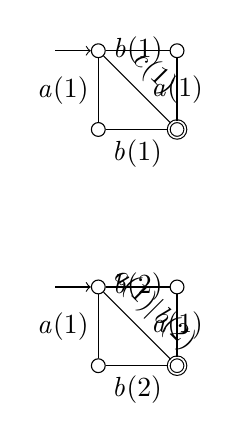
\begin{tikzpicture}
    \tikzstyle{every state}=[
        draw,
        shape=circle,
        inner sep=1pt,
        minimum size=5pt,
        final/.style={double,minimum size=6pt},
        initial text=]

    [->,auto,node distance=1.5cm]
    \renewcommand{\a}[1]{\textit{#1}}
    \node[state] [initial] (n0) {};
    \node[state] [below of=n0] (n1) {};
    \node[state] [right of=n0] (n2) {};
    \node[state, final] [below of=n2] (n3) {};
    \path (n0) edge node[left]{\a{a}(1)} (n1)
            (n0) edge node{\a{b}(1)} (n2)
            (n0) edge node[above=0mm,sloped]{\a{c}(1)} (n3)
            (n1) edge node[below]{\a{b}(1)} (n3)
            (n2) edge node{\a{a}(1)} (n3);

    \begin{scope}[yshift=-3cm]
    \node[state] [initial] (n0) {};
    \node[state] [below of=n0] (n1) {};
    \node[state] [right of=n0] (n2) {};
    \node[state, final] [below of=n2] (n3) {};
    \path (n0) edge node[left]{\a{a}(1)} (n1)
            (n0) edge node{\a{b}(2)} (n2)
            (n0) edge node[above=0mm,sloped]{$\a{a}(1)|\a{b}(2)$} (n3)
            (n1) edge node[below]{\a{b}(2)} (n3)
            (n2) edge node{\a{a}(1)} (n3);
    \end{scope}
\end{tikzpicture}
\end{document}